\section{Results}

We carried out a variety of simulations which involved different countries and available behaviours, as well as different restrictions and valuations applied by our Kyoto Protocol's backbone systems. An individual simulation, with specific configurations regarding which countries are present, what behaviours are being used, and how services act is referred to as a scenario.

\subsection{Possible Scenarios}

During the design and implementation of our Kyoto Protocol simulator, we made any individual simulation configurable in the following ways. This allows us to make sweeping changes to outcomes and agent activities without altering implementation of components of our system. Theoretical alternative scenarios can be contructed in order to test aspects of the real world Kyoto Protocol.

\begin{description}
\item[Session Length] \hfill \\

Session length refers to the number of years in a given commitment period. The longer the sessions, the longer countries will have to meet their target. If this is set too short, countries will be more likely to miss their targets or cheat. This will have repercussions on their ability to spend and invest. They may also choose to just leave the protocol altogether.  The first session of the actual Kyoto Protocol has been extended.

\item[Monitor Price] \hfill \\

The action of monitoing each country has an associated cost. This has been chosen to allow fewer countries than there are in the simulation to be monitored. We were aiming for approximately 10\% of cheating countries to be caught. This was to emulate a more realistic situation where monitoring everyone is not possible, and to allow for countries to cheat and not be caught. However, setting the price to high would reduce the number of countries monitored and lead to cheating becoming an optimal behaviour.

\item[Disabling Monitoring] \hfill \\

The monitor provides a form of insurance against countries cheating. Giving countries free reign over meeting their carbon targets would be a test of the morality in their behaviour. The likely result would be no targets being met and global carbon emissions increasing.

\item[Participants] \hfill \\

Removing the so called `rogue' countries (\textsc{us}) from our simulation would have a large beneficial effect on global emission targets for the remaining participants. This scenario could be compared to a real-world situation where these countries' outputs don't contribute to the way Kyoto set its targets. Although this probably wouldn't help the global carbon emission problem, countries would be more likely to stay if their targets were easier (see Canada).

On the other hand, we could simulate only having `rogue' countries who behave only according to their own internally-set targets. The resulting behaviour would probably be chaotic and not beneficial to the global emission problem. This would be similar to the possible real-world situation where all countries withdraw their support for Kyoto, but commit to their own reduction targets.

The last hypothetical situation we thought would be of interest was if all countries ratified and were classified as Annex 1. Emission targets would be simpler to understand (and fairer compared to the \textsc{us}'s current unrattified status). Also no \textsc{cdm} would take place. This would take away one of the easiest ways for a country to meet their targets while keeping their heavy carbon industry. There is much concern in the real world over the effectiveness and morality of using \textsc{cdm} to reduce carbon emissions. Taking away arable land from third world countries that could be used to grow crops, just to plant trees which will take several decades to become effective carbon sinks sounds very dubious.

\item[CO$_2$ Reduction Rate] \hfill \\

Kyoto aims to reduce the global \CO output by a set amount per session. The faster countries have to reduce their carbon, the more likely they are to miss their target, cheat and/or leave the protocol. We predict a lower reduction rate would be the most beneficial in the long term.


\item[GDP Investment] \hfill \\

Realistically, countries will invest a different proportion of \textsc{gdp} into clean initiatives. Due to countries not needing to worry about spending money on anything non-Kyoto related in our system, we set a fixed percentage to be invested in clean initiatives and industry expansion.   The amount of money a country can spend significantly affects their behaviour.  A lower percentage can cause countries to leave Kyoto as their financial postiion becomes untenable.  Greater percentages may lead to price inflation, or a possiblity of increasing the reduction per year.

\item[GDP Growth] \hfill \\

We have enforced an upper and lower limit on \textsc{gdp} growth of $\pm$-7\%. This reflects the typical real-world values for the majority of stable countries. Increasing this range would make the market more volatile. During growth, investment in industry will have an exaggerated effect, whereas global recession could make it difficult for anyone to meet their targets.

\item[Market State Factors] \hfill \\

These effect the chances of the global economy being in recession or growth, with a weighting towards remaining stable. The state of the market makes industry investment more effective by scaling it.  These could be varied to emulate the protocol during an extended period of either negative or positive growth. The effects would be very similar to changing the \textsc{gdp} growth range as above.
\end{description}

\subsection{Tested Scenarios}

We have a variety of scenarios which have been simulated and run through to completion, with the results then collated and analysed for graphical representation. We attempted to cover a wide variety of Kyoto Protocol environments across our scenarios, while also maintaining baselines for comparison between them. However, we were also limited by the net processing time of running so many scenarios. Running multiple scenarios concurrently, as addressed in the Issues section, presents problems with the MongoDB server, so they must be run relatively sequentially. A single scenario can take up to four hours to run, depending on complexity and number of agents. After execution, the raw data dumped to the database must be processed for representation, which can take up to an additional two hours.

\subsubsection{Real World Scenario}

The real world scenario runs with the default parameters and the full complement of countries. It aims to mirror the real world and the majority of the Kyoto Protocol as accurately as possible, although some variables are approximated, since some values cannot be found, or are not uniform across all countries. Each country has accurate data from 1998 and the simulation runs 40 years from that date.

From our simulation, the data would suggest that the Kyoto Protocol has been a success. Globally, the world has reduced its carbon output by 5081 million tonnes of \CO equivalents, whilst also increasing its overall \textsc{gdp}. The \textsc{us} becomes an Annex I country due to it bringing its emission targets down to a manageable level. The \textsc{us} manages to increase both its \textsc{gdp} and decrease its carbon output at a steady rate, and is perhaps most responsible for the large global decrease in \CO.

However, on closer inspection, the Protocol can be be seen to have harmed the countries who are most responsible for the global decrease in \CO levels. The motion chart shows Annex I countries generally decreasing in \textsc{gdp} as they aim to decrease their carbon output to match their emission targets. The western nations who are the main exponents of Kyoto will refuse to leave the Protocol, and will instead aim to cut down on their industry. This has a detrimental effect on their growth, and pushes many countries into recession.

In contrast, many of the ex-Soviet Bloc countries initially have emission targets well above their current carbon outputs and so can make a significant profit by selling excess credits and reinvesting in their economy. This benefits them throughout the 40 year period, and they correspondingly have a noticeably increase in \textsc{gdp}, and also increase their carbon output. Further to this, these countries are ambivalent towards Kyoto’s aims and so leave when their emissions targets force them to reduce their growth.

Canada is the first Annex country to leave Kyoto. It has a large emissions target and an economy highly dependant on fossil fuels. Interestingly, in this simulation Canada is implemented using the same behaviour code as the countries who are ambivalent towards Kyoto (it is an Annex I sustain agent), but is still the first to leave. This demonstrates that our agent code acts dependent upon its parameterisation and is flexible enough to make intelligent, branching decisions based on its current status in any given scenario. This closely mirrors real world behaviour, as Canada actually left the Kyoto Protocol around 10 years in.

\$785.8B worth of trades were performed in the 40 year period. Trade values vary hugely with a maximum value of \$193421 but an average of \$2611. Trade prices can be falsely inflated by countries hoarding credits until near sanction deadlines and temporarily increasing the price when certain countries are forced to buy.

\textsc{cdm} acts as a stabilising force within the market. Prices for \textsc{cdm} are not set by countries, but are based on the actual cost of their investment. Cost of \textsc{cdm} will increase throughout the game, due to carbon absorption and reduction costs increasing relatively. High demand for \textsc{cdm} will increase the cost faster.

\begin{figure}[H]
		\centering
        \begin{subfigure}[b]{\textwidth}
                \centering
                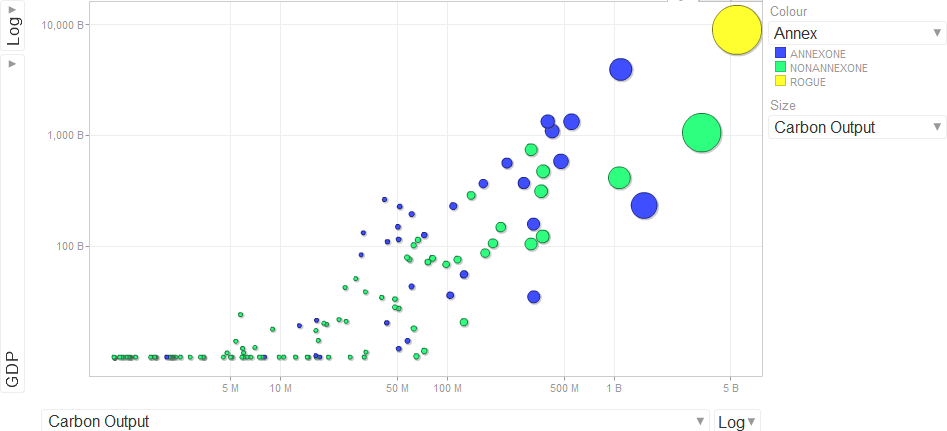
\includegraphics[width=\textwidth]{img/simulations/main-before.png}
				\caption{Data at start of simulation.}
				\label{subfig:main-1}
        \end{subfigure}
        \\
        \begin{subfigure}[b]{\textwidth}
                \centering
                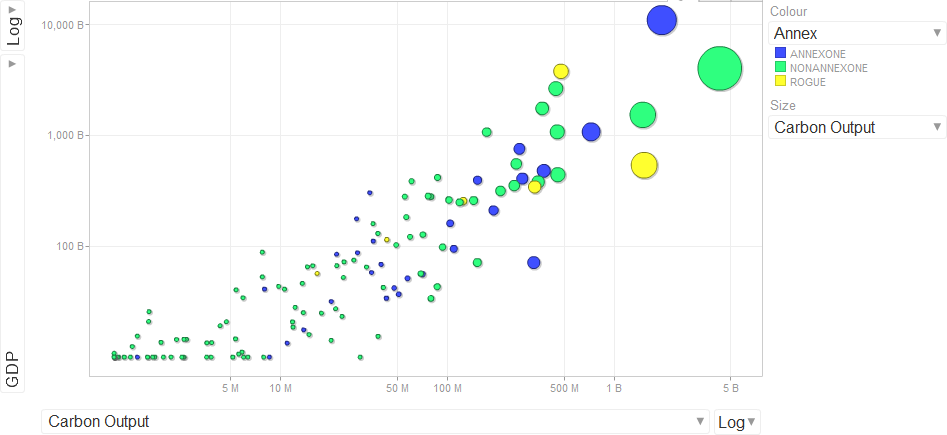
\includegraphics[width=\textwidth]{img/simulations/main-after.png}
				\caption{Data at end of simulation.}
				\label{subfig:main-2}
        \end{subfigure}
        \caption{Results from real world senario}\label{fig:main}
\end{figure}

\subsubsection{Annex I Only}

This simulation only takes countries that are part of Annex I into account, but is otherwise identical to the Real World Simulation.

Non-Annex countries put additional burden on Annex I countries due to their emissions forming part of the global output. Since the former are not set emission targets, they will generally increase their energy and carbon output to help their developing economies. This means stricter emission goals for developed countries, so that the global emissions can still be decreased by 5\% every session. If we remove Non-Annex countries from the simulation, achieving that target becomes significantly easier and cheaper for Annex I countries, as their individual targets are lower.

This behaviour has been evident from the simulation data. With agents being able to meet their targets early on, energy output and \textsc{gdp} would not need to be cut. With countries now able to afford to lower their emissions by means of carbon reduction and absorption, they have enough funds left to invest in industry and increasing their \textsc{gdp}. It is noted that after ~35 years, carbon reduction and absorption becomes prohibitively expensive, and some participants need to scale back their economies to reach their emission targets. Likewise, countries start leaving Kyoto much later than Canada does in the main simulation, with Estonia, Slovakia and Poland being the first to do so in the 38th year.

As a consequence, the global increase of \textsc{gdp} almost doubles compared to the original simulation. There may be two reasons for that:

Allowing developed countries to keep investing in and increasing their economies produces much higher gains than what developing countries can generate, even when they do not need to keep to any targets, or

The economy state - which is random for every simulation - was significantly more favourable for the Annex One only simulation than for the Main simulation.

Another significant difference is the price of obtaining carbon credits. Following the free market rules, removing the option to invest in developing countries in exchange for the credits should decrease their supply on the market, and hence increase their price. However, the existence of United States disrupts that theoretical model completely. They cannot participate in trading, but still have significant funds to spend and a will to contribute to lowering global carbon emissions. Hence, they invest heavily in Non-Annex countries, regardless of the price. This explains why the average price of obtaining carbon credits is almost 4 times lower if \textsc{us} is removed from the simulation.

\textsc{cdm} also acts as a form of price stabiliser since the value of a credit is derived and not determined by the \textsc{ai}.  This can account for the greater deviation in price from the main simulation.

All of the other figures scale linearly with the number of countries being simulated. Global emission target and reduced carbon emissions, as well as the total number of credit trades and their combined value are decreased by a factor of 6-8 comparing to the original simulation, which matches the decrease in number of participating countries.

\begin{figure}[H]
		\centering
        \begin{subfigure}[b]{\textwidth}
                \centering
                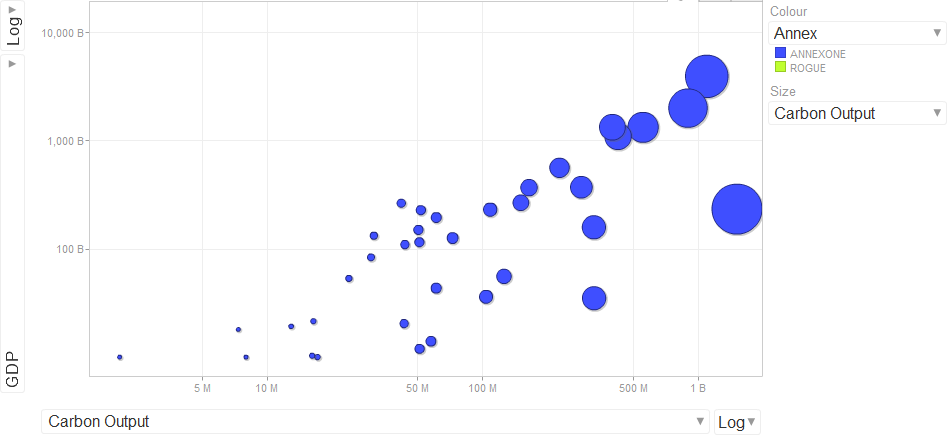
\includegraphics[width=\textwidth]{img/simulations/all-annex1-before.png}
				\caption{Data at start of simulation.}
				\label{subfig:all-annex1-1}
        \end{subfigure}
        \\
        \begin{subfigure}[b]{\textwidth}
                \centering
                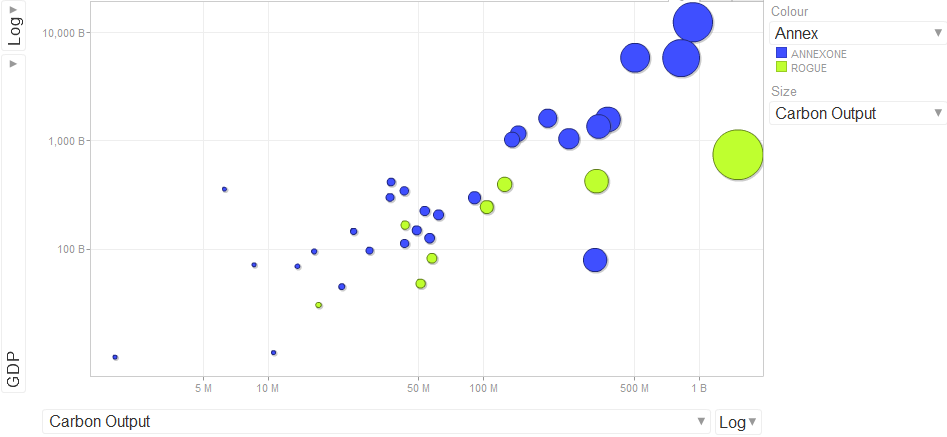
\includegraphics[width=\textwidth]{img/simulations/all-annex1-after.png}
				\caption{Data at end of simulation.}
				\label{subfig:all-annex1-2}
        \end{subfigure}
        \caption{Simulation running only Annex I participants}\label{fig:all-annex1}
\end{figure}

\subsubsection{Comparing Reduction Rates}

We ran a set of three scenarios which used reduction rates of 0.98, 0.95, and 0.92. These scenarios were otherwise identical, so that we could analyse the effect reduction rates have on the efficacy of the Kyoto Protocol.

The two extreme values, 0.98 to 0.92 (hereby known as high and low respectively), differ from the actual Kyoto Protocol. Both of these scenarios present similar global reductions in \CO, which is a lower global reduction than the 0.95 (hereby known as middle) scenario. The high scenario has a lower global reduction for obvious reasons, emissions targets are set higher so countries do not make concerted efforts to reduce their \CO emissions. The reasons for low global emissions reductions in the low scenario, however, are not as immediately obvious. After carefully assessing the scenario, we realized that the harsher target in the low scenario led to larger numbers of countries becoming rogue states more quickly, with their excess emissions offsetting the increased reductions by other Annex I countries.

Global reductions in the high and low scenarios are in the range of 2000 megatonnes. The middle scenario has a global carbon reduction of approximately 5000 megatonnes. From this result we can conclude that the real world reduction targets set out by the Kyoto Protocol lie in an ideal maximum range which will lead to effective global reduction in carbon emissions.

In the low simulation, the first country to go from being an Annex I country to a rogue state does so 12 years after the start of the simulation. In the high scenario, the first country does so after 17 years. This difference demonstrates the variation introduced by the reduction rates.

As can be seen by comparing Figure~\ref{fig:350} and Figure~\ref{fig:352}, the Annex I countries are most drastically affected by more or less severe emissions targets.

\begin{figure}[H]
		\centering
        \begin{subfigure}[b]{\textwidth}
                \centering
                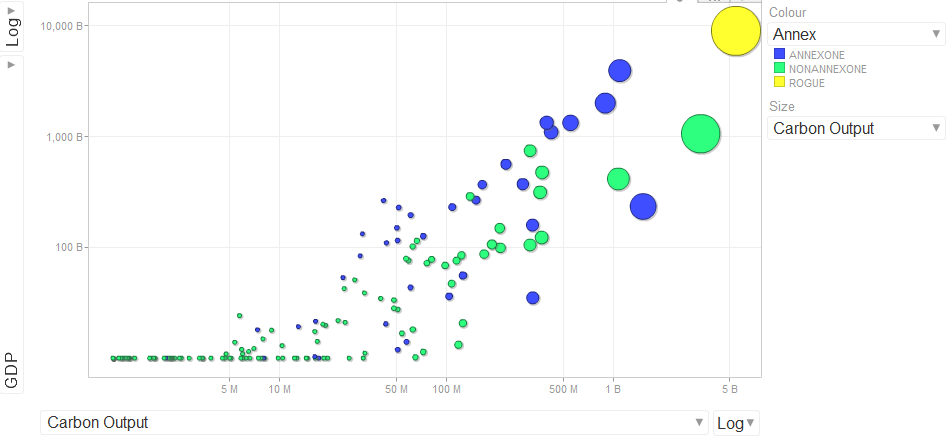
\includegraphics[width=\textwidth]{img/simulations/350-reduction-rate-before.png}
				\caption{Data at start of simulation.}
				\label{subfig:350-1}
        \end{subfigure}
        \\
        \begin{subfigure}[b]{\textwidth}
                \centering
                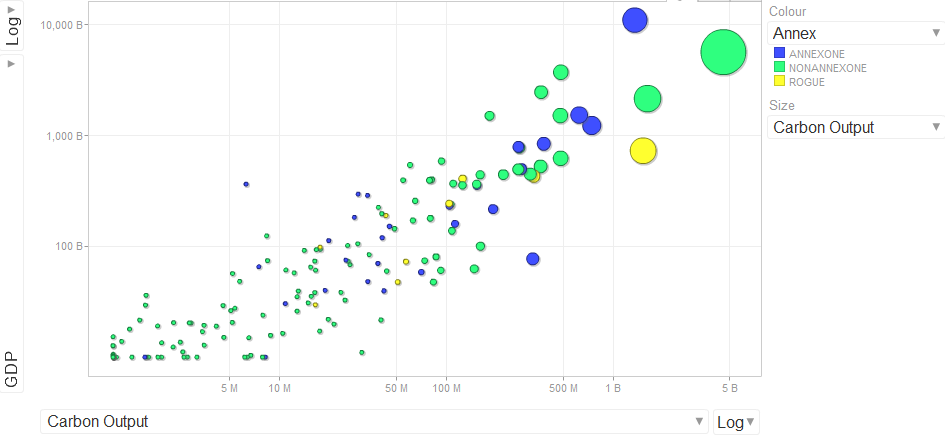
\includegraphics[width=\textwidth]{img/simulations/350-reduction-rate-after.png}
				\caption{Data at end of simulation.}
				\label{subfig:350-2}
        \end{subfigure}
        \caption{Results for simulation ($reduction~rate=0.98$)}\label{fig:350}
\end{figure}

\begin{figure}[H]
		\centering
        \begin{subfigure}[b]{\textwidth}
                \centering
                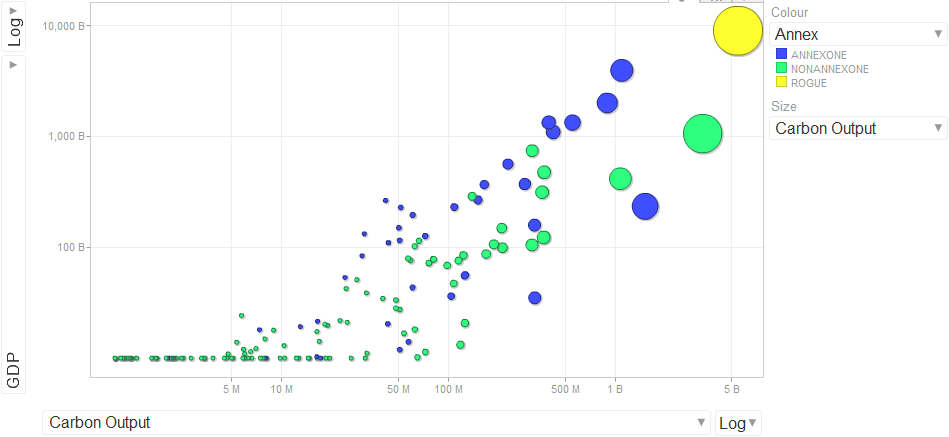
\includegraphics[width=\textwidth]{img/simulations/352-reduction-rate-before.png}
				\caption{Data at start of simulation.}
				\label{subfig:352-1}
        \end{subfigure}
        \\
        \begin{subfigure}[b]{\textwidth}
                \centering
                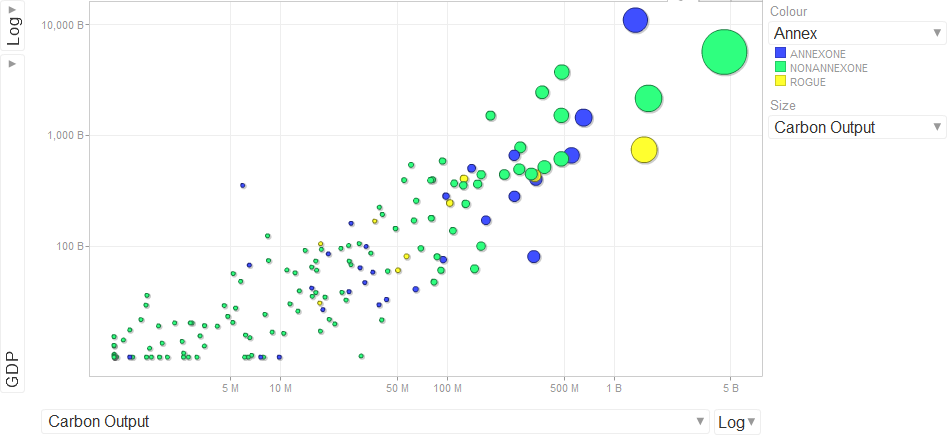
\includegraphics[width=\textwidth]{img/simulations/352-reduction-rate-after.png}
				\caption{Data at end of simulation.}
				\label{subfig:352-2}
        \end{subfigure}
        \caption{Results for simulation ($reduction~rate=0.92$)}\label{fig:352}
\end{figure}

\subsubsection{Recession}

The scenario modelling recession was run with a subset of the total number of countries available. The parameters were chosen such that it would be more likely, at any given time, to have a global recession rather than stability or growth.

Realistically in a recession, countries will increase government spending to get positive economic growth. This particular simulation models the phenomenon quite well. In the subset simulation, countries which were part of the kyoto protocol as Annex I nations faced strict targets, which made it more difficult for them to maintain a stable economic growth in the recession. Figure~\ref{fig:recession}(\ref{subfig:recession-1}) illustrated the initial \textsc{gdp} vs the Carbon Output figures for participants in this simulation.

As the simulation progresses the \textsc{gdp}s of the Annex I countries decrease and a general trend of increasing \textsc{gdp} can be noted in the Non-Annex countries. Non-Annex countries do not get carbon emission targets nor do they get monitored so there are more opportunities for spending in economic expansion with little concern to the carbon output. On the other hand, Annex I countries find it more difficult to meet their targets especially in a difficult global economic condition. An interesting point in the simulation is when Slovakia, an Annex I countries leaves kyoto because of difficulties in meeting the carbon emission targets. At the end of the simulation two countries leave the Kyoto Protocol (Slovakia and Poland). Figure~\ref{fig:recession}(\ref{subfig:recession-2}) The following diagram shows the state of the simulation when the two countries left Kyoto.

\begin{figure}[H]
		\centering
        \begin{subfigure}[b]{\textwidth}
                \centering
                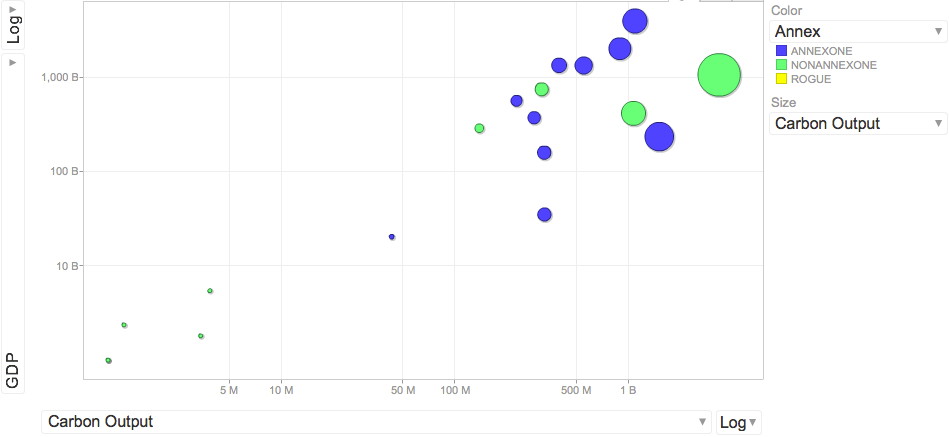
\includegraphics[width=\textwidth]{img/simulations/recession-before.png}
				\caption{Data at start of simulation.}
				\label{subfig:recession-1}
        \end{subfigure}
        \\
        \begin{subfigure}[b]{\textwidth}
                \centering
                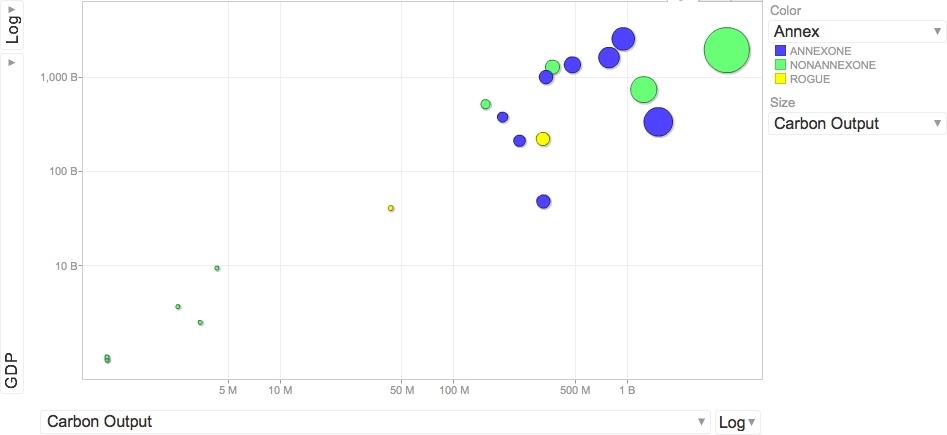
\includegraphics[width=\textwidth]{img/simulations/recession-after.png}
				\caption{Data at end of simulation.}
				\label{subfig:recession-2}
        \end{subfigure}
        \caption{Results for simulation (recession)}\label{fig:recession}
\end{figure}

The total carbon emission reduction totalled to -411 tonnes, which is an expected result when countries spend more in the economic growth with little concern to the carbon output.

\textsc{cdm} is a cheaper alternative for countries to increase their carbon offsets. In the simulation there was a total of 449 \textsc{cdm} investments. This is expected as it is a viable route for countries which are concerned about keeping their carbon emissions below the emission target.

In more complex simulations it can be seen that the total carbon emission reduction is quite large, if this simulation was run with more countries then the collaborative contribution from other countries would perhaps give a positive reduction as opposed to the one originally obtained for the simulation.
